\section{Experimental Results}
\label{experiment}

\subsection{Dataset}
\label{experiment:dataset}
We experiment on five trajectory datasets, four of them were provided by \cite{ijcai15}.
Trajectories in these datasets were extracted from Yahoo! Flickr Creative Commons 100M
(a.k.a. YFCC100M) dataset\cite{thomee2016yfcc100m} using metadata of photos and videos
such as geographical locations, timestamps, user identifications etc,
the details of building trajectories are covered in \cite{ht10} and \cite{ijcai15} and
we refer interested readers to these papers.
Statistics of the four trajectory datasets are described in table \ref{table:data}.
%
The time that a user arrived a POI was approximated by the time the first photo taken by the user at that POI,
similarly, the time that a user leaved a POI was approximated by the time the last photo taken by the user at
that POI \cite{ht10, ijcai15}.
An example of trajectory with four POIs from Toronto dataset was shown in figure \ref{fig:traj},
%TODO: explain what is a POI/photo in the figure
where the four colored marker icons represent the four POIs,
and the colored round icons represent a sample of photos assign to these POIs.


\begin{figure}
\centering
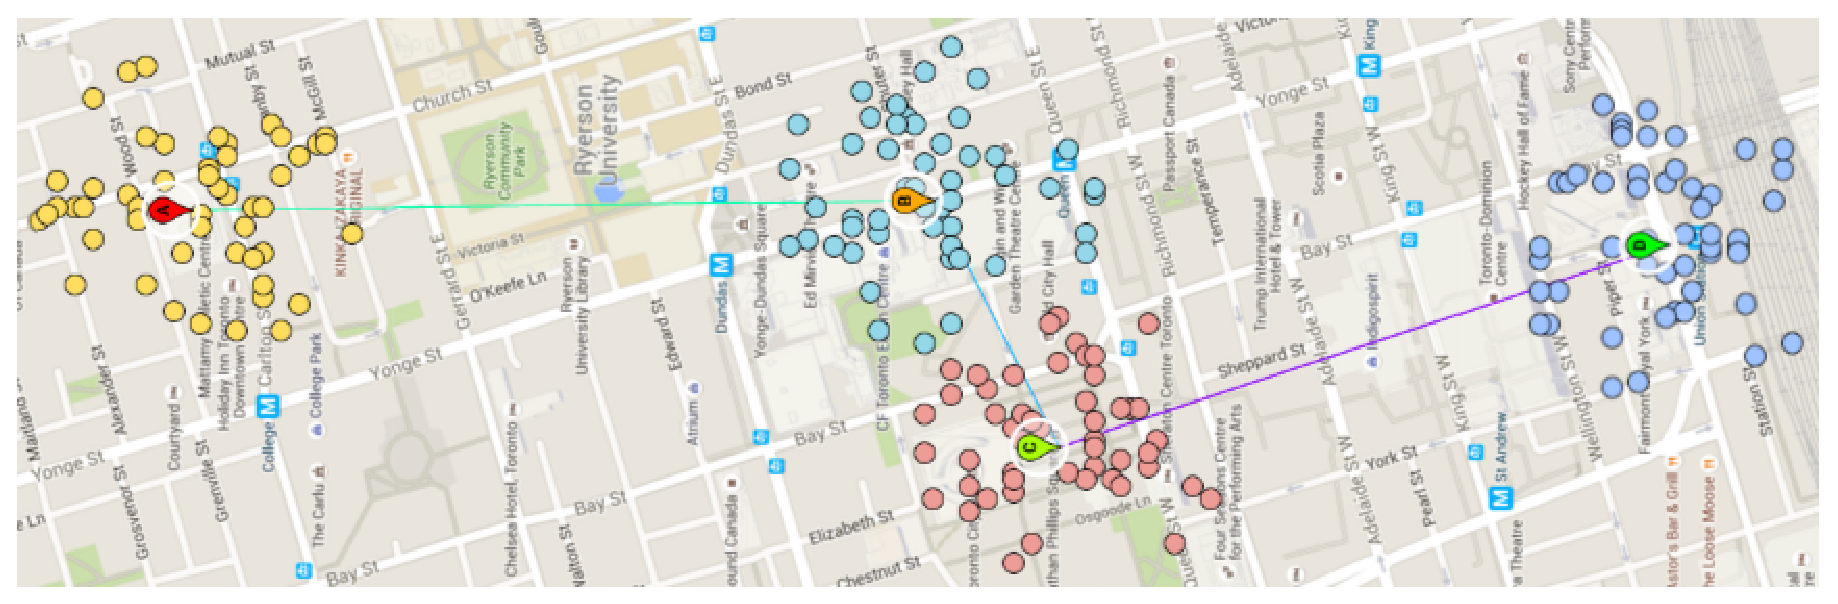
\epsfig{file=fig/traj_eg.eps, width=3.5in}
\caption{An example of trajectory with four POIs}
\label{fig:traj}
\end{figure}

\begin{table*}
\centering
\begin{tabular}{lrrrrr} \hline
\textbf{Dataset} & \textbf{\#Photos} & \textbf{\#POI Visits} & \textbf{\#Trajectories} & \textbf{\#Users} \\ \hline
Edinburgh & 82,060 & 33,944 & 5,028 & 1,454 \\
Glasgow & 29,019 & 11,434 & 2,227 & 601 \\
Melbourne & 94,142 & 23,995 & 5,106 & 1,000 \\
Osaka & 392,420 & 7,747 & 1,115 & 450 \\
Toronto & 157,505 & 39,419 & 6,057 & 1,395 \\
\hline
\end{tabular}
\caption{Statistics of trajectory dataset}
\label{table:data}
\end{table*}


\subsection{Performance metric}
\label{sec:metric}

\cheng{Let's try this here. Still needs polishing.}

To evaluate the performance of different trajectory recommendation algorithms,
we employ the trajectory F$_1$-score\cite{ijcai15} to measure the POIs that are
correctly recommended. Let $\mathcal{T}$ be the trajectory that was visited in the real world,
and $\hat{\mathcal{T}}$ be the recommended trajectory,
$\mathcal{P}_{\mathcal{T}}$ be the set of POIs visited in $\mathcal{T}$,
and $\mathcal{P}_{\hat{\mathcal{T}}}$ be the set of POIs visited in $\hat{\mathcal{T}}$,
trajectory F$_1$-scores was defined as
\begin{displaymath}
    F_1 = \frac{2 |\mathcal{P}_{\mathcal{T}} \cap \mathcal{P}_{\hat{\mathcal{T}}}|}
               {|\mathcal{P}_{\mathcal{T}}| + |\mathcal{P}_{\hat{\mathcal{T}}}|}
\end{displaymath}

A perfect trajectory F$_1$-score (i.e., F$_1 = 1$) means the POIs in the recommended trajectory are exactly
the same POIs as those in the ground truth, and a $0$ trajectory F$_1$-score means that unfortunately none of
the POIs in the real trajectory was recommended.

In addition, to measure the quality of recommended visiting order of POIs,
we propose a new metric $F_{1,\textsc{order}}$,
\begin{displaymath}
F_{1,\textsc{order}} = \frac{2 \times P_{\textsc{order}} \times R_{\textsc{order}}}
                           {P_{\textsc{order}} + R_{\textsc{order}}}
\end{displaymath}
where
\begin{displaymath}
P_{\textsc{order}} = \frac{N_c} {|\hat{\mathcal{T}}|(|\hat{\mathcal{T}}|-1) / 2},
R_{\textsc{order}} = \frac{N_c} {|\mathcal{T}|(|\mathcal{T}|-1) / 2}
\end{displaymath}
and $N_c$ is the number of POI pairs $(p_j, p_k)$ that satisfies the following
constraints\footnote{We define $F_{1,\textsc{order}}=0$ if $N_c$ is $0$.}:
\begin{align*}
    (p_j \prec_{\mathcal{T}} p_k ~\land~ p_j \prec_{\hat{\mathcal{T}}} p_k) & ~\lor~
    (p_j \succ_{\mathcal{T}} p_k ~\land~ p_j \succ_{\hat{\mathcal{T}}} p_k) \\
    p_j \ne p_k, &~~ p_j, p_k \in \mathcal{P}_{\mathcal{T}} \cap \mathcal{P}_{\hat{\mathcal{T}}} \\
    j \ne k, &~~ 1 \le j, k \le |\mathcal{T}|
\end{align*}

A perfect trajectory $F_{1,\textsc{order}}$, i.e., $F_{1,\textsc{order}} = 1$, means that both the POIs and their visiting order in the
recommended trajectory are exactly the same as these in the real trajectory,
and $F_{1,\textsc{order}} = 0$ means that none of the recommended POI pairs was actually visited in the real trajectory.


\subsection{Experimental Setup}
We use leave-one-out cross validation to evaluate different trajectory recommendation algorithms,
i.e., when evaluating a trajectory of a specific user, all other trajectories of this user as well as
all trajectories of other users were used to train the recommendation algorithms.

We conducted a comprehensive benchmark to compare the performance of different recommendation approaches.
In addition to the \textsc{PoiPopularity}, we also applied the \textsc{Random} baseline which naively chooses 
POIs uniformly at random (without replacement) from the set of POIs $\mathcal{P} \setminus \{p_s, p_e \}$ to visit.

Among the related approaches, \textsc{PersTour}\cite{ijcai15} is the most similar one, it formulated 
trajectory recommendation as an Orienteering Problem and use integer linear programming to maximise 
an objective, which composes both the POI popularity and user interest at the recommended POIs.
A user's interest on a specific category of POIs is modelled as the total ratios of his/her actual visit duration 
over the average visit duration at these POIs in general.
The recommended trajectory was also constrained by a time budget besides the origin and destination POIs.
To make further comparison, we replace the time budget in \textsc{PersTour} with the trajectory length and
denote this algorithm as \textsc{PersTour-L}.

Other recommendation approaches in this benchmark including \textsc{PoiRank} which utilises the ranking of POIs
described in section \ref{sec:ranksvm}, and \textsc{Markov} that recommending trajectories uses only transition 
probabilities between POIs, as described in section \ref{sec:transition}. Its variant \textsc{MarkovPath} that incorporates 
sub-tour elimination constraints described in section \ref{sec:walkpath} is also included.
Furthermore, \textsc{Rank+Markov} algorithm that leverage both POI ranking and transition probabilities as well as
its non-sub-tour variant \textsc{Rank+MarkovPath} that detailed in section \ref{sec:recommendation} are also 
benchmarked.

Lastly, we have the \textsc{StructuredSVM} that not only utilises POI ranking and transition probabilities but also 
jointly optimises their relative importance, as described in section \ref{sec:ssvm}.
The information that captured by these algorithms is summarised in table \ref{tab:characteristic},
and the associated parameters of these algorithms are detailed in the appendix.


\begin{table}
\centering\small
\begin{tabular}{l|cccccc} \hline
                                    & Query    & POI      & Trans. & No sub- & Joint    \\
                                    &     &       &  & tours &     \\ \hline
\textsc{Random}                     & $\times$ & $\times$ & $\times$   & $\times$     & $\times$ \\
\textsc{PersTour}\cite{ijcai15}     & $\times$ & $\surd$  & $\times$   & $\surd$      & $\times$ \\
\textsc{PersTour-L}                 & $\times$ & $\surd$  & $\times$   & $\surd$      & $\times$ \\
\textsc{PoiPopularity}              & $\times$ & $\surd$  & $\times$   & $\times$     & $\times$ \\
\textsc{PoiRank}                    & $\surd$  & $\surd$  & $\times$   & $\times$     & $\times$ \\
\textsc{Markov}                     & $\times$ & $\surd$  & $\surd$    & $\times$     & $\times$ \\
\textsc{MarkovPath}                 & $\times$ & $\surd$  & $\surd$    & $\surd$      & $\times$ \\
\textsc{Rank}+\textsc{Markov}     & $\surd$  & $\surd$  & $\surd$    & $\times$     & $\times$ \\
\textsc{Rank}+\textsc{MarkovPath} & $\surd$  & $\surd$  & $\surd$    & $\surd$      & $\times$ \\
\textsc{StructuredSVM}              & $\surd$  & $\surd$  & $\surd$    & $\times$     & $\surd$  \\ \hline
\end{tabular}
\caption{Characteristics of different algorithms}
\label{tab:characteristic}
\end{table}


\subsection{Results}
% tell the story: justify each row in the table, make comparison.
The F$_1$-scores of the nine algorithms on all four datasets are shown in table \ref{table:f1}.
The information utilized by these algorithms except \textsc{Random} range from POI specific and query specific
information to transition patterns between different POIs and so on, as is shown in table \ref{tab:characteristic}.

From table \ref{table:f1}, one can observe that all algorithms that capture POI specific information
outperform the one that does not use it, namely the \textsc{Random} baseline algorithm,
with one exception of \textsc{PersTour} on Melbourne dataset,
which indicates the POI specific information is very helpful for recommending trajectories.
%
% time constraint is better than length constraint
Another observation is \textsc{PersTour} get much better trajectory F$_1$-scores on four out of five datasets
than \textsc{PersTour-L}, which is equivalent to \textsc{PersTour} except the total number of POIs was used to
constrain recommendation, which means the total time consumed in a trajectory was more helpful than the number
of POIs one should visit.
%
% comparison between ijcai and other methods
However, algorithms that did not utilise the total time consumed in a trajectory can outperform the one that
used this information (i.e., \textsc{PersTour}) on four out of five datasets,
by learning to rank POIs based on POI specific and query specific features and exploiting the transition patterns
between POIs.

% strong performance of POI popularity based ranking on Edinburgh data
POI features seem to be very helpful for recommending trajectories.
In particular, recommendation based on ranking POI popularity only
(i.e., \textsc{PoiPopularity}) yields very good performance,
especially on Edinburgh dataset, where it surprisingly outperforms all
other algorithms, including those much more sophisticated than this simple ranking method.
%
% strong performance of POI feature based ranking on Toronto and Glasgow data
Furthermore, \textsc{PoiRank} performs very well in four out of five datasets,
especially on Toronto and Melbourne datasets, where it got better results than any other methods,
while on both Edinburgh and Glasgow datasets, it was the second best performer,
which indicates that learning to rank is very helpful for recommending trajectories.

% the performance of transition-only methods
Recommendation by exploiting only transition patterns did not performs quite well,
but when supported by learning to rank, it improves a lot, which results the best performer on Osaka dataset
and the second or third best performer on all other datasets, namely \textsc{Rank+MarkovPath}.

% sub-tours hurt
In addition, we found that sub-tours hurt trajectory recommendation when compare the performance between
algorithms with or without sub-tours restrictions, namely, \textsc{Markov} versus \textsc{MarkovPath} and
\textsc{Rank+Markov} versue \textsc{Rank+MarkovPath}.
%
% why structured prediction didn't work very well
This discovery could also be the reason that the sophisticated structured prediction algorithm,
i.e., \textsc{StructuredSVM}, since it utilised the same features as both \textsc{Rank+Markov} and
\textsc{Rank+MarkovPath}, but only got comparable or slightly better results than \textsc{Rank+Markov}
and cannot outperform \textsc{Rank+MarkovPath} on four out of five datasets, and was only doing slightly
better on Toronto dataset, even it took advantage of a significantly larger number of parameters.

% performance comparison in terms of tau
On the other hand, when compare the performance of different recommendation algorithms in terms of trajectory $\tau$
which try to measure the quality of visiting orders of POIs in recommended trajectories,
as shown in table \ref{table:tau}
\footnote{We can not compute trajectory $\tau$ for \textsc{PersTour} because the number of POIs in recommend trajectory
is not guaranteed to equal the number of POIs in real trajectory.},
\textsc{StructuredSVM} became the best performer in three out of five datasets,
this is not unexpected as \textsc{StructuredSVM} can tune much more parameters than any other algorithms when training,
which means it can utilise the transition patterns between POIs better,
as a result, when POIs in a recommended trajectory also appear in the ground truth,
there is a better chance that the visiting order among these POIs are also consistent with
that in the real trajectory.

%
The last interesting observation that we want to point out is the performance of ranking based algorithms
on Edinburgh, Glasgow and Toronto datasets, when measured in terms of both trajectory F$_1$ score and trajectory
$\tau$, \textsc{PoiPopularity} performed very well on Edinburgh dataset, and \textsc{PoiRank} yielded very good
performance on both Glasgow and Toronto datasets.
This observation indicates that most tourists visiting these three cities not only just visiting
places that are very popular, but also following similar visiting orders when visiting these places.


\begin{table*}
\centering
\begin{tabular}{l|ccccc} \hline
 & Edinburgh & Glasgow & Melbourne & Osaka & Toronto \\ \hline
\textsc{Random} & $0.570\pm0.139$ & $0.632\pm0.124$ & $0.558\pm0.149$ & $0.621\pm0.117$ & $0.621\pm0.128$ \\
\textsc{PersTour}\cite{ijcai15} & $0.656\pm0.223$ & $\mathbf{0.802\pm0.213}$ & $0.491\pm0.211$ & $0.702\pm0.230$ & $0.720\pm0.215$ \\
\textsc{PersTour-L} & $0.651\pm0.143$ & $0.660\pm0.102$ & $0.578\pm0.140$ & $0.691\pm0.138$ & $0.642\pm0.112$ \\
\textsc{PoiPopularity} & $\mathbf{0.701\pm0.160}$ & $0.745\pm0.166$ & $0.621\pm0.136$ & $0.661\pm0.128$ & $0.679\pm0.120$ \\
\textsc{PoiRank} & $\mathit{0.694\pm0.157}$ & $\mathit{0.777\pm0.171}$ & $\mathbf{0.626\pm0.137}$ & $0.679\pm0.112$ & $\mathbf{0.748\pm0.166}$ \\
\textsc{Markov} & $0.629\pm0.172$ & $0.714\pm0.168$ & $0.577\pm0.168$ & $0.679\pm0.162$ & $0.663\pm0.157$ \\
\textsc{MarkovPath} & $0.678\pm0.148$ & $0.735\pm0.170$ & $0.596\pm0.147$ & $0.706\pm0.154$ & $0.689\pm0.140$ \\
\textsc{Rank+Markov} & $0.642\pm0.171$ & $0.736\pm0.176$ & $0.598\pm0.169$ & $0.701\pm0.171$ & $0.689\pm0.170$ \\
\textsc{Rank+MarkovPath} & $0.684\pm0.151$ & $0.760\pm0.170$ & $\mathit{0.625\pm0.150}$ & $\mathbf{0.719\pm0.161}$ & $0.724\pm0.152$ \\
\textsc{StructuredSVM} & $0.659\pm0.186$ & $0.727\pm0.173$ & $0.597\pm0.171$ & $\mathit{0.715\pm0.170}$ & $\mathit{0.728\pm0.186}$ \\
\hline
\end{tabular}
\caption{Performance comparison on four datasets in terms of trajectory F$_1$-score.
         For each dataset (i.e., a column), the best method is shown in bold, the second best is shown in italic.}
\label{table:f1}
\end{table*}


\begin{table*}
\centering
\begin{tabular}{l|ccccc} \hline
 & Edinburgh & Glasgow & Melbourne & Osaka & Toronto \\ \hline
\textsc{Random} & $0.261\pm0.155$ & $0.320\pm0.169$ & $0.249\pm0.148$ & $0.305\pm0.145$ & $0.311\pm0.167$ \\
\textsc{PersTour}\cite{ijcai15} & $0.417\pm0.343$ & $\mathbf{0.646\pm0.366}$ & $0.225\pm0.274$ & $\mathit{0.491\pm0.377}$ & $0.503\pm0.353$ \\
\textsc{PersTour-L} & $0.359\pm0.207$ & $0.352\pm0.162$ & $0.268\pm0.143$ & $0.415\pm0.243$ & $0.331\pm0.159$ \\
\textsc{PoiPopularity} & $\mathit{0.436\pm0.259}$ & $0.509\pm0.299$ & $0.316\pm0.178$ & $0.363\pm0.195$ & $0.385\pm0.202$ \\
\textsc{PoiRank} & $0.424\pm0.249$ & $\mathit{0.565\pm0.312}$ & $0.322\pm0.186$ & $0.376\pm0.173$ & $\mathit{0.512\pm0.295}$ \\
\textsc{Markov} & $0.424\pm0.238$ & $0.488\pm0.283$ & $0.297\pm0.192$ & $0.449\pm0.262$ & $0.419\pm0.237$ \\
\textsc{MarkovPath} & $0.400\pm0.234$ & $0.492\pm0.298$ & $0.294\pm0.187$ & $0.445\pm0.268$ & $0.407\pm0.234$ \\
\textsc{Rank+Markov} & $0.434\pm0.251$ & $0.540\pm0.294$ & $\mathbf{0.357\pm0.210}$ & $0.483\pm0.277$ & $0.462\pm0.266$ \\
\textsc{Rank+MarkovPath} & $0.408\pm0.239$ & $0.532\pm0.304$ & $0.331\pm0.213$ & $0.470\pm0.284$ & $0.465\pm0.266$ \\
\textsc{StructuredSVM} & $\mathbf{0.440\pm0.267}$ & $0.529\pm0.283$ & $\mathit{0.352\pm0.213}$ & $\mathbf{0.508\pm0.292}$ & $\mathbf{0.520\pm0.311}$ \\
\hline
\end{tabular}
\caption{Performance comparison on four datasets in terms of $\tau$.
         For each dataset (i.e., a column), the best method is shown in bold, the second best is shown in italic.}
\label{table:tau}
\end{table*}




\subsection{Avoid Peeking}
When working with machine learning algorithms, to make sure the reported performance is a good approximation
of the generalization performance, it is critical to prevent information in test set from leaking into
training set.
Many algorithms in the above comparison utilizing both learning to rank and factorized transition matrix,
e.g., \textsc{Rank+Markov}, \textsc{Rank+MarkovPath} and \textsc{StructuredSVM},
both of them need to be trained or parameters be estimated before being utilized in other algorithms.
Features such as popularity of a POI, the number of visits of a POI and the average visit duration at a POI are
determined by not only the POI itself but also trajectories in training set, let's call them aggregated features as they are
computed by aggregating a set of trajectories.
To make sure the prediction performance is reliable, it is very important to exclude trajectories in test set
when computing aggregated features.
Unfortunately, it is quite easy, especially when utilizing multiple levels of machine learning models,
to use all data, including those in test set, to compute aggregated features and many researchers and
practitioners did not realize some bits of information in test set were leaked into training set via these aggregated features.

%One may argue that many of these features will not change much when computed with or without data in test set,
%but in certain areas, such as aerodynamics, some decisions are very sensitive to the quantity of certain features.
%Nevertheless, the exact impact still needs further investigation.
